%{\color{red}[VJ note: We need to move part of this into the evaluation section. Otherwise, it looks good]}
\label{sec:access}
The SERUMS user authentication scheme will go beyond traditional "one-size-fits-all" practices towards adopting a personalised and adaptable multi-factor user authentication scheme which will be based on a flexible authentication paradigm, coined FlexPass \cite{belk,constantinides,hadjidemetriou}. A first conceptual design of the proposed flexible user authentication paradigm is depicted in Figure \ref{fig:flexpass}. Our approach attempts to provide a new user authentication paradigm that leverages upon theories in Cognitive Psychology (dual coding, episodic and semantic memory), which suggest that humans' episodic and semantic memories, represented as verbal and visual information, can be transformed into memorable and personal authentication secrets. Such secrets can be semantically similarly reflected on both textual and graphical password keys, and accordingly used complimentary based on user preference (Figure \ref{fig:flexpass}) \cite{belk}. The paradigm relies on a single, open-ended, user-selected secret that can be reflected as a textual key and a graphical key. 

\begin{figure}[H]
    \centering
    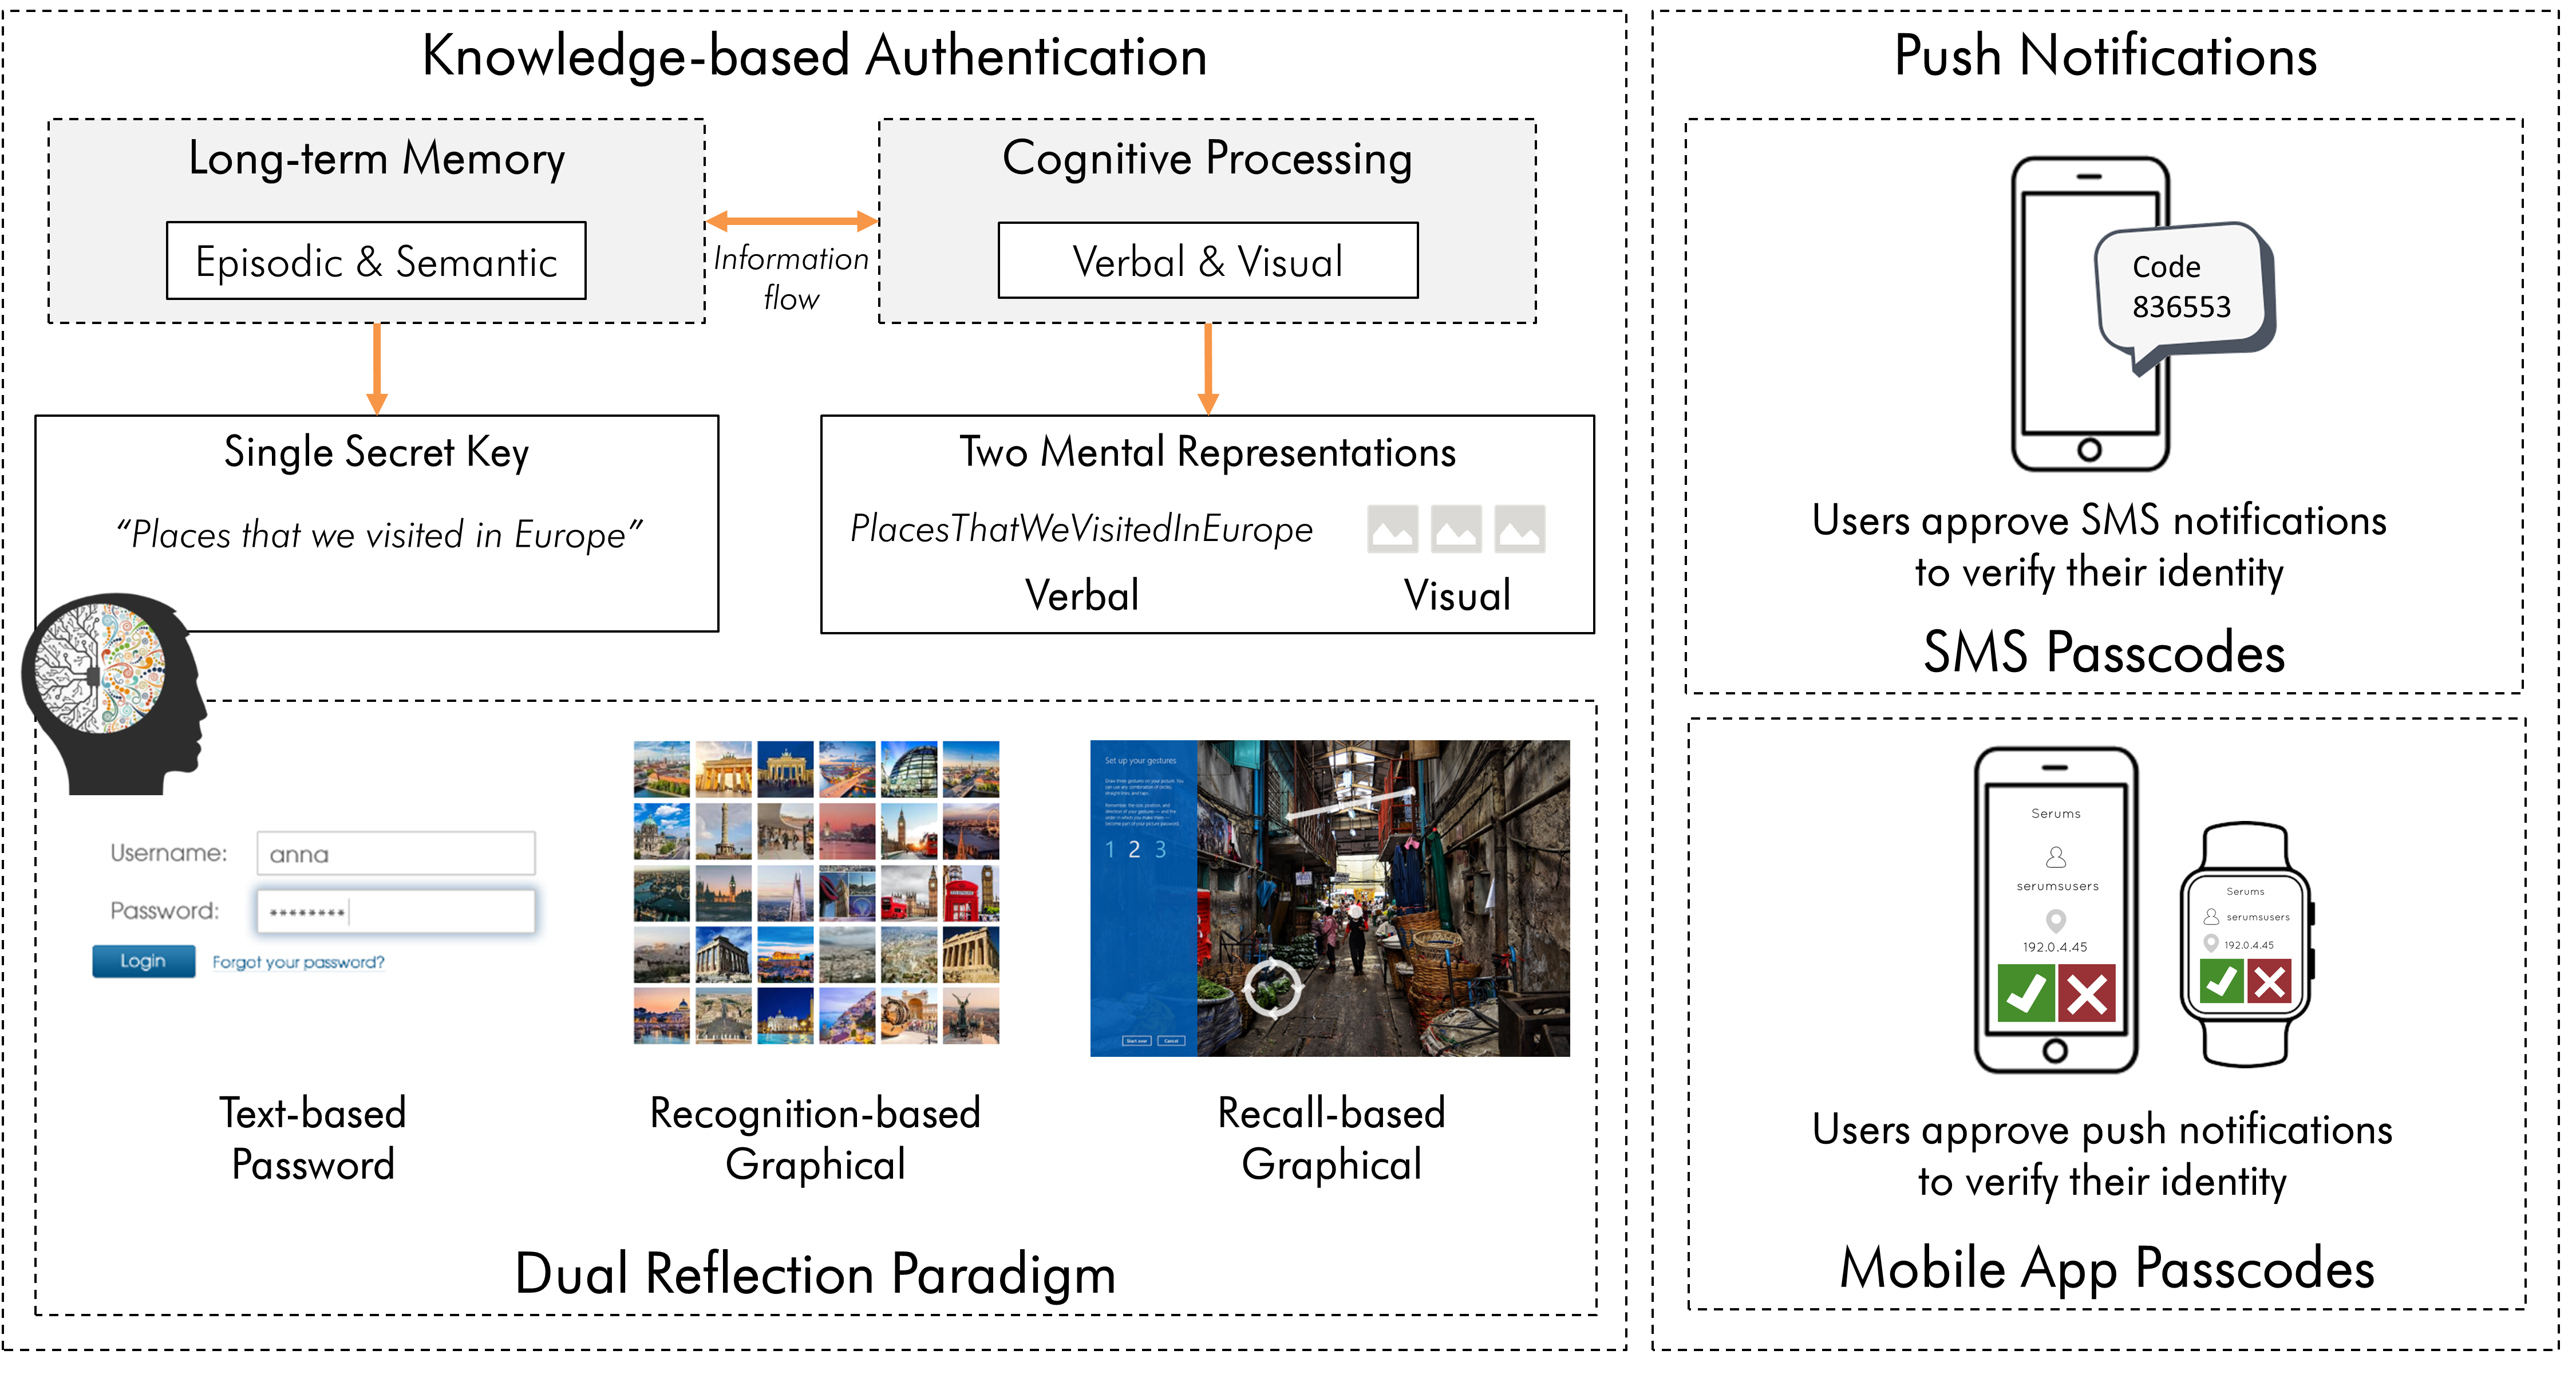
\includegraphics[width=90mm]{images/flexpass.png}
    \caption{Conceptual design of the Flexible User Authentication Paradigm}
    \label{fig:flexpass}
\end{figure}

The FlexPass paradigm extends existing works in knowledge-based user authentication based on theories of human cognition with the aim: a) to enhance memorability through ownership, and prior experience and knowledge of each single user; and b) to support user authentication adaptability since users can choose their preferred way to login based on their needs and context of use. For example, users that are on the move and interact on their smartphone might prefer to login with a graphical password, instead of entering text on a virtual keyboard which is considered a demanding and time-consuming task \cite{vonzezschwitz}. The same user however, in a different context, e.g., while at home working on the desktop computer, can choose to login through his textual password key. Note that in both cases, the user is only required to recall the same single secret, which can be reflected differently based on the user’s preference. Similarly, older adults might prefer to always login with a graphical password since they find it easier than textual passwords, as opposed to younger adults that instead, prefer traditional textual passwords \cite{nicholson}.

Nevertheless, the dual nature of FlexPass embraces new security vulnerabilities that need to be addressed, i.e., it introduces a new observational attack since adversaries can see the set of pictures (user-selected and decoy images) during login. A brute-force algorithm could use such information from the graphical representation to guess the secret. Aiming to add an additional layer of security, we use a second factor for authentication through push notifications as a first step before proceeding to login. In particular, at a first stage users will be required to approve a push notification that is realised as an SMS notification including an OTP, and a mobile application notification. After verifying their identity, users will login through their preferred user authentication type based on the FlexPass paradigm. Furthermore, the open-ended nature of the paradigm might affect users towards misuse strategies. To assure that users will not create semantically insecure (predictable) grids of images, automated image tagging technologies and policies need to be investigated to prevent users’ unsafe coping strategies. 